\section{Kalibrierung}

\subsection{Energie}

Um aus der am PC ausgegebenen Kanalzahl die entsprechende Neutronenenergie bestimmen zu können, muss zunächst eine Kalibrierung durchgeführt werden. Da die Kanallagen aus den in den Szintillatoren gemessenen Elektronenenergien stammen, muss zunächst ein Zusammenhang zwischen der Kanalnummer und der Elektronenenergie hergestellt werden:

\begin{align}
E_e=a+b\cdot K
\end{align}

Dafür wird das $\gamma$-Spektrum der $^{22}Na$-Quelle aufgenommen und die Lage der beiden Compton-Kanten bestimmt. Um später das korrekte Energiespektrum (Neutronenenergie bis ca. 10MeV) zu messen, muss hierbei auf die passende Einstellung der Elektronik geachtet werden, welche durch äußere Einflüsse, wie Wärme und Feuchtigkeit beeinflusst wird. Die gewählten Einstellungen finden sich in \ref{para}. 

\begin{table}[h]
	\caption{Messparameter der Energiekalibrierung}
	\begin{tabular}{|c|c|c|}
	\hline
	 Coarse Gain & Fine Gain & Messdauer\\ \hline
	 100 & 0,75 & 3512s\\ \hline
	\end{tabular}
\label{para}
\end{table}

Die beiden Compton-Kanten entsprechen $\gamma$-Quanten mit 511 bzw. 1275 keV, welche aus den Übergängen der Quelle stammen. Über die in der Theorie beschriebene Formel, kann die zugehörige Elektronenergie bestimmt werden:

\begin{align}
E_{e,1}=\frac{2\alpha \cdot E_{\gamma}}{1 + 2\alpha} = \frac{2\cdot \frac{511keV}{511keV}\cdot 511keV}{1+2\cdot \frac{511keV}{511keV}}=\frac{2\cdot 511keV}{3}\approx 340,7keV
\end{align}
\begin{align}
E_{e,2}=\frac{2\alpha \cdot E_{\gamma}}{1 + 2\alpha} = \frac{2\cdot \frac{1275keV}{511keV}\cdot 1275keV}{1+2\cdot \frac{1275keV}{511keV}}=\approx 1062,2keV
\end{align}

Die aus dem Spektrum bestimmten Compton-Kanten befinden sich bei den Kanälen 68 bzw. 202. Aus den Werten und dem gerade beschriebenen Elektron-Photon Zusammenhang ergibt sich die Eichung zu:

\begin{align}
b= \frac{1062,2-340,7}{202,5-68} \approx 5,36 \frac{keV}{K}
\end{align}
\begin{align}
a=340,7-b\cdot 68 \approx -24,1 keV
\end{align}
\begin{align}
E_e=-24,1 keV +5,36 \frac{keV}{K} \cdot K
\end{align}

Die maximale Elektronenenergie ergibt sich über die maximale Kanalnummer von 1024 zu:

\begin{align}
E_{e,max}=-24,1 + 5,36 \cdot 1024 \approx 5470 keV 
\end{align}

Über die in Abbildung \ref{E-N} dargestellte Beziehung der Elektronen- und Neutronenenergien lässt sich das messbare Energiespektrum der Neutronen bestimmen, was in unserem Fall Neutronen bis ungefähr 11 MeV umfasst. 

\begin{figure}[htbp]  
     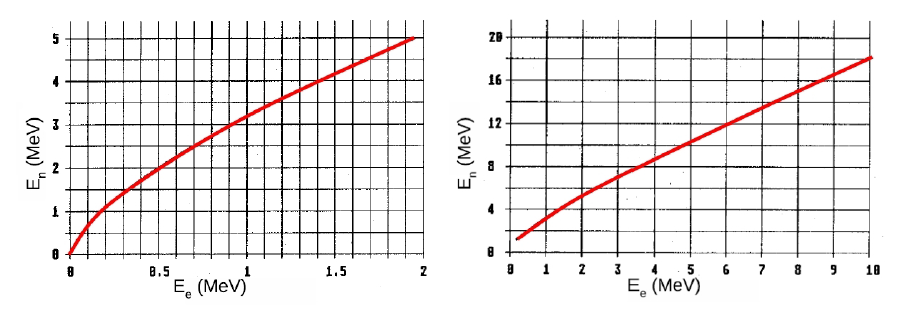
\includegraphics[width=1\textwidth]{E-N.png}
  \caption{Energiebeziehung Elektronen - Neutronen \cite{anleitung}}
  \label{E-N}
\end{figure}

\subsection{Time of Flight}

Für die später folgende Time-of-Flight(ToF)-Messung muss nun auch eine Kalibrierung der Kanalzahl in Flugzeit durchgeführt werden. Die im ToF-Spektrum angezeigten Daten entsprechen dabei der zeitlichen Differenz zwischen den beiden Detektoren, wobei je größer die Differenz, desto höher die Kanalnummer gilt. Um die Kanaldifferenz später auch in Zeitdifferenz umrechnen zu können, muss folgende Kalibrierung bestimmt werden:

\begin{align}
\Delta t = a \cdot \Delta K
\end{align}

Dafür wird das gleiche Spektrum zweimal aufgenommen und die Lagen zweier Peaks im ToF-Spektrum bestimmt, wobei bei der zweiten Messung über eine Delay-Box ein künstliches Delay von 30ns zugeschaltet wird. Dadurch verschiebt sich das gesamte Spektrum hin zu höheren Kanalnummern und die Kalibrierung kann bestimmt werden. Die Messzeit beträgt in beiden Fällen 960s. Die bestimmten Kanallagen finden sich in \ref{ToF}, für jeden Peak einmal ohne zusätzliches Delay  (o.D.) und einmal mit einem Delay von 30ns (m.D.)

\begin{table}[h]
	\caption{Kanallagen der Peaks im ToF-Spektrum}
	\begin{tabular}{|c|c|c|c|}
	\hline
	 Peak 1 o.D. & Peak 2 o.D. & Peak 1 m.D. & Peak 2 m.D.\\ \hline
	 465 & 493 & 762 & 786\\ \hline
	\end{tabular}
\label{ToF}
\end{table}

Die Kalibrierung des ToF-Spektrums ergibt sich nun zu:

\begin{align}
a=\frac{\Delta t}{\Delta K}=\frac{30ns}{762 - 465} = \frac{30ns}{786 - 493} \approx 0,101 \frac{ns}{K}
\end{align}



 